% <!-- coding: utf-8 -->
\renewcommand{\monlhead}{Données ornitho faune-bretagne}
\section*{Présentation}
Les données sont extraites de faune-bretagne sur la zone géographique -1.775795/48.105037 -1.711859/48.060601

Cette extraction est faite en format csv. Les données sont ensuite traitées en R

Un rapprochement est effectué avec le référenciel taxonomique TAXREF.
Les espèces spécifiques à biolovision ne sont pas prises en compte.

Les familles sont différentes pour certaines espèces, en version 9.0 de TAXREF :
\begin{itemize}
\item Roitelet à triple bandeau   Sylviidae   Regulidae
\item Rougegorge familier    Turdidae Saxicolidae
\end{itemize}

Des statistiques sont produites pour :
\begin{itemize}
\item les données sur la zone d'extraction
\item les données sur la période 1er décembre 2016 - 20 janvier 2017
\end{itemize}
\section*{Statistiques données antérieures}
\subsection*{par famille}
\includegraphics[width=\malargeurgraphique]{images/faune_prec_stat_champ_FAMILY_NAME.pdf}
\subsection*{par année}
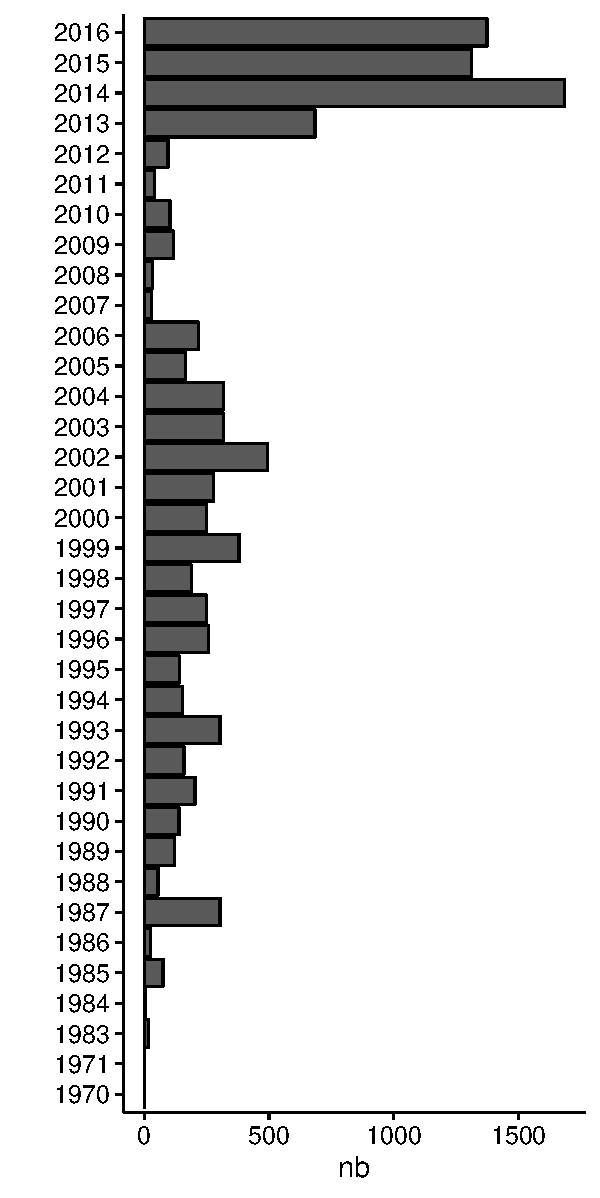
\includegraphics[width=\malargeurgraphique]{images/faune_prec_stat_champ_annee.pdf}
\subsection*{par mois}
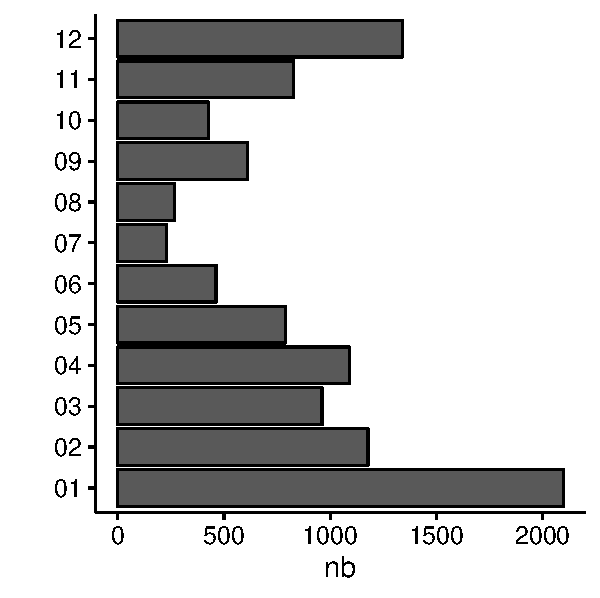
\includegraphics[width=\malargeurgraphique]{images/faune_prec_stat_champ_mois.pdf}
\subsection*{par type de localisation}
\includegraphics[width=\malargeurgraphique]{images/faune_prec_stat_champ_PRECISION.pdf}
\section*{Statistiques 1er décembre 2016 - 20 janvier 2017}
\subsection*{par famille}
\includegraphics[width=\malargeurgraphique]{images/faune_stat_champ_FAMILY_NAME.pdf}
\subsection*{par famille taxref}
\includegraphics[width=\malargeurgraphique]{images/faune_stat_champ_FAMILLE.pdf}
\subsection*{par ordre taxref}
\includegraphics[width=\malargeurgraphique]{images/faune_stat_champ_ORDRE.pdf}
\subsection*{par espèce}
\includegraphics[width=\malargeurgraphique]{images/faune_stat_champ_NAME_SPECIES.pdf}
\subsection*{par date}
\includegraphics[width=\malargeurgraphique]{images/faune_stat_champ_d.pdf}
\subsection*{par observateur}
\includegraphics[width=\malargeurgraphique]{images/faune_stat_champ_observateur.pdf}
\subsection*{par lieudit}
\includegraphics[width=\malargeurgraphique]{images/faune_stat_champ_PLACE.pdf}
\subsection*{par type de localisation}
\includegraphics[width=\malargeurgraphique]{images/faune_stat_champ_PRECISION.pdf}
\clearpage
\section*{Carte}
\includegraphics[width=\textwidth]{images/faune_carte.pdf}